\lstset{ %
	language=C,                % Язык программирования                % где поставить нумерацию строк (слева\справа)
	numberstyle=\tiny,           % размер шрифта для номеров строк
	stepnumber=1,                   % размер шага между двумя номерами строк
	numbersep=5pt,                % как далеко отстоят номера строк от подсвечиваемого кода
	showspaces=false,            % показывать или нет пробелы специальными отступами
	showstringspaces=false,      % показывать или нет пробелы в строках
	showtabs=false,             % показывать или нет табуляцию в строках
	tabsize=2,                 % размер табуляции по умолчанию равен 2 пробелам
	captionpos=t,              % позиция заголовка вверху [t] или внизу [b] 
	breaklines=true,           % автоматически переносить строки (да\нет)
	breakatwhitespace=false,       
	frame=single,                    % Добавить рамку
	basicstyle=\small,
	escapebegin=\begin{russian}\commentfont,
		escapeend=\end{russian},
	literate={Ö}{{\"O}}1
	{Ä}{{\"A}}1
	{Ü}{{\"U}}1
	{ß}{{\ss}}1
	{ü}{{\"u}}1
	{ä}{{\"a}}1
	{ö}{{\"o}}1
	{~}{{\textasciitilde}}1
	{а}{{\selectfont\char224}}1
	{б}{{\selectfont\char225}}1
	{в}{{\selectfont\char226}}1
	{г}{{\selectfont\char227}}1
	{д}{{\selectfont\char228}}1
	{е}{{\selectfont\char229}}1
	{ё}{{\"e}}1
	{ж}{{\selectfont\char230}}1
	{з}{{\selectfont\char231}}1
	{и}{{\selectfont\char232}}1
	{й}{{\selectfont\char233}}1
	{к}{{\selectfont\char234}}1
	{л}{{\selectfont\char235}}1
	{м}{{\selectfont\char236}}1
	{н}{{\selectfont\char237}}1
	{о}{{\selectfont\char238}}1
	{п}{{\selectfont\char239}}1
	{р}{{\selectfont\char240}}1
	{с}{{\selectfont\char241}}1
	{т}{{\selectfont\char242}}1
	{у}{{\selectfont\char243}}1
	{ф}{{\selectfont\char244}}1
	{х}{{\selectfont\char245}}1
	{ц}{{\selectfont\char246}}1
	{ч}{{\selectfont\char247}}1
	{ш}{{\selectfont\char248}}1
	{щ}{{\selectfont\char249}}1
	{ъ}{{\selectfont\char250}}1
	{ы}{{\selectfont\char251}}1
	{ь}{{\selectfont\char252}}1
	{э}{{\selectfont\char253}}1
	{ю}{{\selectfont\char254}}1
	{я}{{\selectfont\char255}}1
	{А}{{\selectfont\char192}}1
	{Б}{{\selectfont\char193}}1
	{В}{{\selectfont\char194}}1
	{Г}{{\selectfont\char195}}1
	{Д}{{\selectfont\char196}}1
	{Е}{{\selectfont\char197}}1
	{Ё}{{\"E}}1
	{Ж}{{\selectfont\char198}}1
	{З}{{\selectfont\char199}}1
	{И}{{\selectfont\char200}}1
	{Й}{{\selectfont\char201}}1
	{К}{{\selectfont\char202}}1
	{Л}{{\selectfont\char203}}1
	{М}{{\selectfont\char204}}1
	{Н}{{\selectfont\char205}}1
	{О}{{\selectfont\char206}}1
	{П}{{\selectfont\char207}}1
	{Р}{{\selectfont\char208}}1
	{С}{{\selectfont\char209}}1
	{Т}{{\selectfont\char210}}1
	{У}{{\selectfont\char211}}1
	{Ф}{{\selectfont\char212}}1
	{Х}{{\selectfont\char213}}1
	{Ц}{{\selectfont\char214}}1
	{Ч}{{\selectfont\char215}}1
	{Ш}{{\selectfont\char216}}1
	{Щ}{{\selectfont\char217}}1
	{Ъ}{{\selectfont\char218}}1
	{Ы}{{\selectfont\char219}}1
	{Ь}{{\selectfont\char220}}1
	{Э}{{\selectfont\char221}}1
	{Ю}{{\selectfont\char222}}1
	{Я}{{\selectfont\char223}}1
	{і}{{\selectfont\char105}}1
	{ї}{{\selectfont\char168}}1
	{є}{{\selectfont\char185}}1
	{ґ}{{\selectfont\char160}}1
	{І}{{\selectfont\char73}}1
	{Ї}{{\selectfont\char136}}1
	{Є}{{\selectfont\char153}}1
	{Ґ}{{\selectfont\char128}}1
}
\newpage
\section*{Задание}
\addcontentsline{toc}{section}{\tocsecindent{Задание}}

\Large В информационный центр приходят клиенты через интервал времени 10 $\pm$ 2 минуты. Если все три имеющихся оператора заняты, клиенту отказывают в обслуживании. Операторы имеют разную производительность и могут обеспечивать обслуживание среднего запроса пользователя за 20 $\pm$ 5; 40 $\pm$ 10; 40 $\pm$ 20. Клиенты стремятся занять свободного оператора с максимальной производительностью. Полученные запросы сдаются в накопитель. Откуда выбираются на обработку. На первый компьютер запросы от 1 и 2-ого операторов, на второй -- запросы от 3-его. Время обработки запросов первым и 2-м компьютером равны соответственно 15 и 30 мин. Промоделировать процесс обработки 300 запросов. 

Необходимо для этого создать концептуальную модель в терминах СМО (рис.1), определить эндогенные и экзогенные переменные и уравнения модели. За единицу системного времени выбрать 0,01 минуты. 

Найти вероятность отказа, используя язык GPSS.

\begin{figure}[h]
	\center{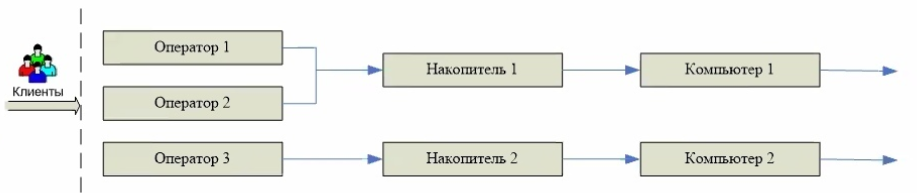
\includegraphics[width=1\linewidth]{img/1} \\ $\Delta t=1, p = 99\%$}
	\caption{Концептуальная модель}
	\label{ris:image1}
\end{figure}

\newpage

\section*{Листинг кода}
\addcontentsline{toc}{section}{\tocsecindent{Листинг кода}}
Ниже представлен листинг кода программы:
\begin{figure}[h]
	\center{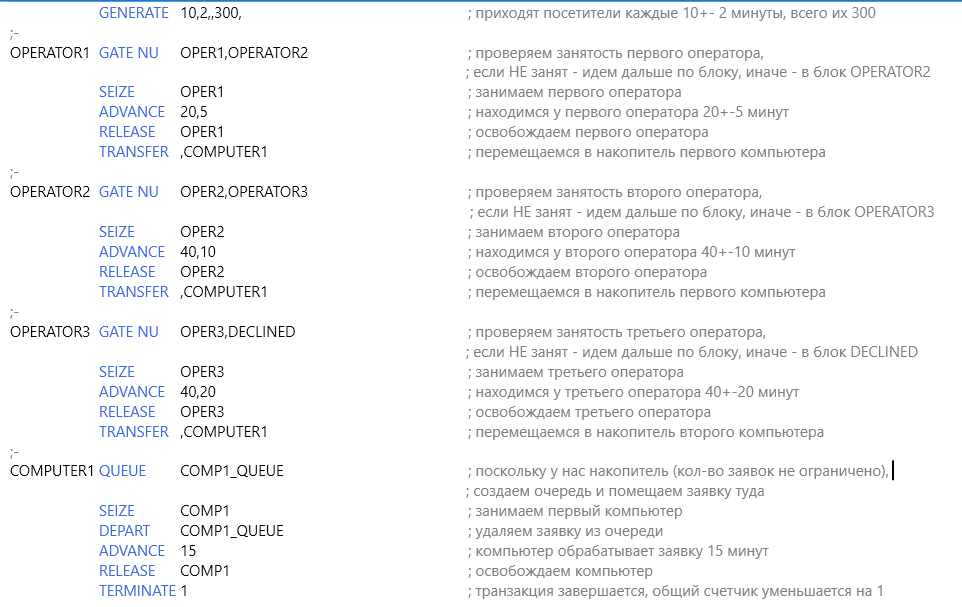
\includegraphics[width=0.99\linewidth]{img/2} \\ }
	\label{ris:image1}
\end{figure}
\begin{figure}[h]
	\center{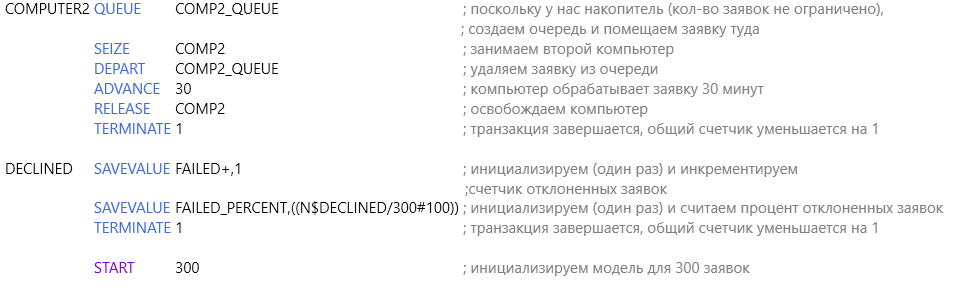
\includegraphics[width=0.99\linewidth]{img/4} \\ }
	\label{ris:image1}
\end{figure}
\newpage
\section*{Результаты работы}
\addcontentsline{toc}{section}{\tocsecindent{Результаты работы}}
Ниже представлены результаты работы программы при 300 запросах:

\begin{figure}[h]
		\center{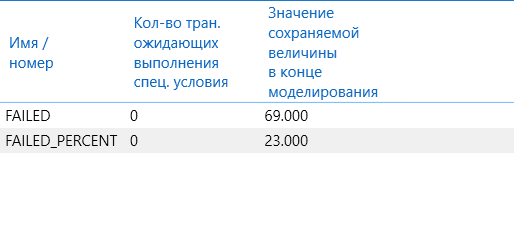
\includegraphics[width=0.45\linewidth]{img/3} \\ }
	\caption{Количество отклоненных заявок (FAILED) и вероятность этого отказа (FAILED\_PERCENT)}
	\label{ris:image1}
\end{figure}


\section*{Вывод}
\addcontentsline{toc}{section}{\tocsecindent{Вывод}}
Была разработана программа на языке GPSS, моделирующая информационный центр, состоящий из генератора заявок, двух накопителей, трех операторов и двух компьютеров. Результатом работы является количество клиентов, получивших отказ и вероятность этого отказа.